\documentclass{article}

\usepackage[T1]{fontenc}
\usepackage{graphicx}
\usepackage{fancyhdr}
\pagestyle{fancy}
\fancyhf{}
\lhead{Version 1.0}
\rhead{Elliot Oram}
\rfoot{\thepage}


\title{Overall System Activity Diagram}
\author{elo9@aber.ac.uk}

\begin{document}

\maketitle
\tableofcontents

\newpage

\section{Activity diagram}
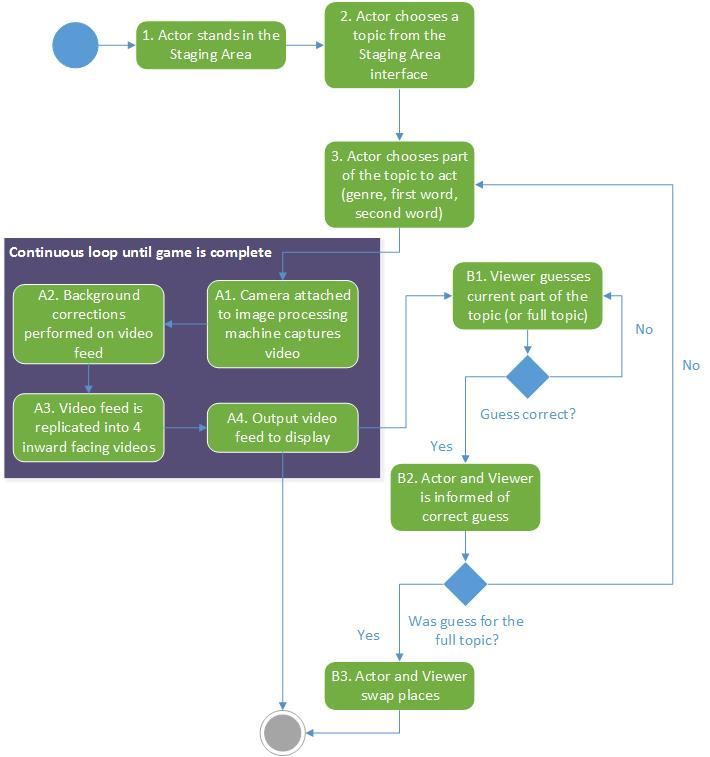
\includegraphics[width=\textwidth]{SystemActivityDiagramImage}

\newpage


\section{Description of Activity Diagram}
\begin{itemize}
	\item [1] First Actor is chosen from the Viewers. This can be done by someone volunteering or at random. Additional system functionality could be added to support choosing the first Actor.
	
	\item [2] The Actor is given the choice of 5 phrases random selected by the system and enters their desired phrase to act via the Staging Area interface. \textit{(Staging interface will be tablet or similar).}
	
	\item [3] The Actor chooses the word of the phrase they wish to act first. This will either be a number for the corresponding word or an option to act the full phrase.
	
	\item [4] The Genre of the phrase being acted (book, film, television show) as well as the current word being acted, is displayed to the Viewer. The Viewer will be in the Viewing area \textit{(where the hologram is being displayed)}.
	
	\item [5] A prompt to begin the image processing loop will be sent to the image processing machine. This will turn the camera on (if it is not already).  
	
	\item \textbf{Image processing loop}

	\subitem [A1] The camera is part of the Staging Area and points at the actor. The camera will be a peripheral of the image processing machine.
	
	\subitem [A2] The image processing application will perform background subtraction on the camera feed to ensure the background of the video is completely black (remove lighting noise ect.).
	
	\subitem [A3] The video feed will be duplicated into 4 versions of itself and formatted appropriately to work with the Pepper's Ghost Pyramid in the Viewing Area. There will be a copy of the video feed on each side of the pyramid, where all videos face inwards towards the centre of the pyramid.
	
	\subitem [A4] The video feed is sent to the displaying area.
	
	\item \textbf{Game loop}	
	
	\subitem [B1] The Viewer attempts to guess the current word or full phrase being acted by looking at the hologram. The guess will be entered on an interface device (tablet or similar) in the Viewing Area. There may be several tablets available for multiple users.
	
	\subitem [B2] If the guess is correct, then the Viewers and Actor are informed on their respective interface device.
	
	\subitem [B3] If the full phrase has been guessed and the game has finished (reached the full number of rounds). A prompt is sent to the image processing machine to stop the processing loop and the game finishes.
	
	\subitem [B4] If the full phrase has been guessed but the game is not over, the Actor is told to swap places with the Viewer who guessed correctly. The system then returns to the initial state.
	
	
\end{itemize}

\end{document}